%%%%%%%%%%%%%%%%%%%%%%%%%%%%%%%%%%%%%%%%%%%%%%%%%%%%%%%%%%%%%%%%%%%%%%%%%%%%%%%%
%2345678901234567890123456789012345678901234567890123456789012345678901234567890
%        1         2         3         4         5         6         7         8

\documentclass[letterpaper, 10 pt, conference]{ieeeconf}  % Comment this line out if you need a4paper

%\documentclass[a4paper, 10pt, conference]{ieeeconf}      % Use this line for a4 paper

\IEEEoverridecommandlockouts                              % This command is only needed if 
                                                          % you want to use the \thanks command

\overrideIEEEmargins                                      % Needed to meet printer requirements.

%In case you encounter the following error:
%Error 1010 The PDF file may be corrupt (unable to open PDF file) OR
%Error 1000 An error occurred while parsing a contents stream. Unable to analyze the PDF file.
%This is a known problem with pdfLaTeX conversion filter. The file cannot be opened with acrobat reader
%Please use one of the alternatives below to circumvent this error by uncommenting one or the other
%\pdfobjcompresslevel=0
%\pdfminorversion=4

% See the \addtolength command later in the file to balance the column lengths
% on the last page of the document

% The following packages can be found on http:\\www.ctan.org
\usepackage{graphics} % for pdf, bitmapped graphics files
\usepackage{epsfig} % for postscript graphics files
\usepackage{algorithm}
\usepackage{algpseudocode}
%\usepackage{align}
%\usepackage{mathptmx} % assumes new font selection scheme installed
%\usepackage{times} % assumes new font selection scheme installed
%\usepackage{amsmath} % assumes amsmath package installed
%\usepackage{amssymb}  % assumes amsmath package installed

\title{\LARGE \bf
A Hybrid Control Framework for Autonomous Vehicles at Uncontrolled Intersections}


\author{Nitin R. Kapania$^{1}$, Francesco Borrelli, J Christian Gerdes% <-this % stops a space
\thanks{*This work was supported by the Hyundai Center of Excellence}% <-this % stops a space
\thanks{$^{1}$Nitin Kapania is with the Dept. of Mechanical Engineering, Stanford University, and is a visiting scholar at UC Berkeley}%
}


\begin{document}



\maketitle
\thispagestyle{empty}
\pagestyle{empty}


%%%%%%%%%%%%%%%%%%%%%%%%%%%%%%%%%%%%%%%%%%%%%%%%%%%%%%%%%%%%%%%%%%%%%%%%%%%%%%%%
\begin{abstract}

As autonomous vehicles (AVs) inch closer to reality, a central requirement for acceptance will be earning the trust of humans in everyday driving situations. In particular, the interaction between AVs and pedestrians is of
high importance, as every human is a pedestrian at some point of the day. This paper considers the interaction of a pedestrian and an autonomous vehicle at a mid-block, uncontrolled intersection where there is ambiguity
over when the pedestrian should cross and when and how the vehicle should yield. By modeling pedestrian behavior through the concept of gap acceptance, the authors show that a hybrid controller with just four distinct modes allows an autonomous vehicle to successfully interact with a pedestrian across a continuous spectrum of possible crosswalk-entry behaviors. The controller is validated in simulation through comparison with a previously published control policy obtained through solution of a POMDP, and experimental results are provided on a Hyundai Genesis vehicle for a virtual pedestrian.  

\end{abstract}


%%%%%%%%%%%%%%%%%%%%%%%%%%%%%%%%%%%%%%%%%%%%%%%%%%%%%%%%%%%%%%%%%%%%%%%%%%%%%%%%
\section{Introduction}

\subsection{Motivation}

While autonomous vehicles have the potential to save thousands of lives every year and create tremendous societal benefits \cite{Fagnant2015}, widespread adoption is unlikely until AVs gain the broad trust of society. Given that every human is a pedestrian at some point during the day, one of the central ways that autonomous vehicles will be evaluated is through their interactions with pedestrians. In fact, recent events with industry leader Waymo highlight that AV-pedestrian interaction has still not been perfected\cite{MattRichtelandConorDougherty2015}. In general, interactions with pedestrians are complex, even for experienced human drivers. Issues such as lack of visibility, improper communication, poorly marked roads, and distraction on both the driver or pedestrian side can lead to accidents and fatalities. From 2015-2016, pedestrian fatalaties increased by 9\% to 5987, representing the highest number since 1990, and also representing 16\% of all automotive fatalities \cite{HighwayTrafficSafetyAdministration2016}. As autonomous vehicles inch closer to widespread adoption, they must have a clear control strategy for pedestrian interaction that can handle a wide variety of pedestrian behaviors while maintaining a reasonable flow of traffic.    

\subsection{Prior Art}

The need to further understand pedestrian behavior for autonomous driving has created a growing body of interdisciplinary research. One branch of research has focused around modeling pedestrian behavior given various sensor inputs. Keller et al \cite{Keller2014} presented a study on pedestrian path prediction and action classification (e.g. crossing vs. waiting) using Gaussian process dynamical models and trajectory matching from optical data. Several other techniques for pedestrian trajectory prediction have been proposed, including LQR \cite{Batkovic}, set-based reachability analysis \cite{Koschi2018}, and Markov processes \cite{Karasev2016} 

Another branch of literature is focused on developing predictive models for pedestrian crossing. While typically studied for purposes of road design, this body of literature holds promising insights for AV designers. For example, Schroeder and Rouphail \cite{Schroeder2011} explored factors associated with driver yielding behavior at unsignalized pedestrian crossings. Using logistic regression, the authors found that drivers are more likely to yield to assertive pedestrians who walk briskly in their approach to a crosswalk. Kadali and Perumal \cite{RaghuramKadali2012} studied the ``gap acceptance" behavior of pedestrians at mid-block crosswalks through a video graphic survey, and found that the gap accepted for crossing was explained by factors such as crossing direction, vehicle speed, and pedestrian age. Yannis et al. \cite{Yannis2013} and \cite{Sun2002} also found that gap acceptance was influenced by the size of the oncoming vehicle and the presence of other pedestrians.  Lee and Aty \cite{Lee2005} studied interactions in the form of crashes, and found crashes were linked with higher daily traffic. 

Finally, a small but rapidly growing body of literature specifically studies the interaction between pedestrians and autonomous vehicles at crosswalks. An excellent review of these studies was conducted by \cite{Rasouli}. As an example, Rothenbucher et al. \cite{Rothenbucher2016} studied the interaction between pedestrians and driverless vehicles by constructing a car seat costume to disguise a driver. The authors noted that pedestrians overall managed interactions at crosswalks effectively, but later mentioned increased uncertainty about the autonomous vehicles behavior. To improve the issue of trust, several researchers have developed external interfaces to more clearly broadcast the intent of the autonomous vehicle \cite{Matthews}, \cite{Lagstrom2015}. 

Several real-world studies of AV-pedestrian interaction note that once a local population learned a vehicle was programmed to be perfectly safe, pedestrians would regularly take advantage of the AV and walk in front of it. \cite{Madigan}. This illustrates an issue with automated driving in that an overly conservative crossing algorithm will often be taken advantage of or cause confusion among pedestrians. Camara et al \cite{Camara2018} attempted to model the natural negotation for priority between a pedestrian and an AV at an intersection using the framework of ``sequential chicken" adopted from game theory. Chen et al. \cite{Chen} notes the need for a tradeoff between passive and aggressive driving behavior, and developed a stochastic model of pedestrian behavior to evaluate proposed AV control policies. Control polices for pedestrian interaction are also developed by \cite{Bandyopadhyay}, who proposes a Mixed-observable Markov Decision Process (MOMDP) to incorporate the intention uncertainty of a pedestrian. A POMDP formulation is also proposed by Thornton \cite{Thornton2018}, who proposes navigation of the pedestrian uncertainty through value-sensitive design. 

\subsection{Statement of Contributions}
Significant research has been conducted to understand the likelihood of pedestrian crossing given certain traffic conditions and pedestrian demographics \cite{Schroeder2011} -\cite{Lee2005}, and a small but growing body of literature develops control strategies for pedestrian avoidance \cite{Bandyopadhyay}-\cite{Thornton2018}. However, what is missing is a contribution that explicitly  tests whether a proposed control strategy is robust to the variety of pedestrian behaviors that have been observed from experimental studies on real roads. What is also missing is analysis of how this controller should behave across multiple traffic scenarios - for example, the navigation problem is different for the pedestrian crossing on the opposing side of traffic, and also depends on which particular lane the vehicle is in.   

This paper aims to address this gap by developing a hybrid control architecture that accounts for several distinct pedestrian modes of behavior at an unsignalized crosswalk. An unsignalized crosswalk is chosen as it is the trickiest crosswalk for a pedestrian and vehicle to navigate, as there is no explicit declaration of whose turn it is cross. Simulations show that the state machine controller is able to handle a continuous spectrum of pedestrian \textit{gap acceptance} behavior, tolerating a range of highly conservative to highly aggressive pedestrians. Moreover, this is possible with just four distinct states. Simulations are also used to compare the closed-loop controller with the controller developed by \cite{Thornton2018}. Finally, experimental results are shown on a real vehicle to demonstrate the feasibility of the proposed state machine controller. 


\section{Problem Overview}

\subsection{Unsignalized Intersections}

In general, pedestrian crosswalks may be controlled or uncontrolled. In the case of the former, control devices such as stop signs or walk signals guide the interaction of vehicles and pedestrians explicitly. Fig.~\ref{fig:schematic} shows the latter example, in which a pedestrian must select a gap in traffic flow and cross.   

\begin{figure}
\centering
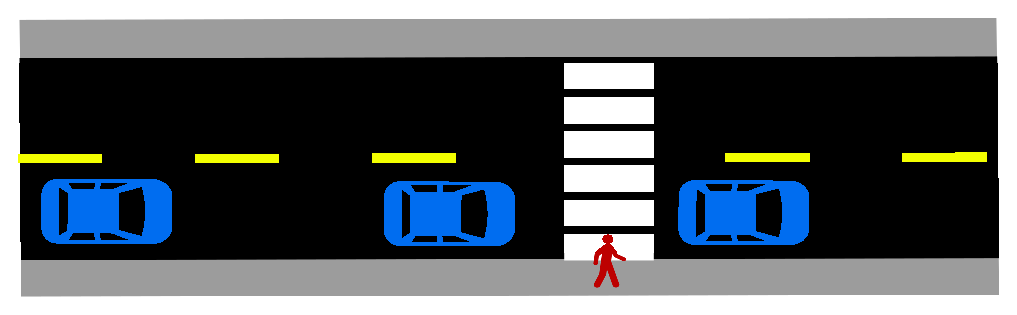
\includegraphics[width=3.5in]{figures/example.eps}
\caption{Schematic of pedestrian approaching a stream of traffic at a mid-block intersection.}
\label{fig:schematic}
\end{figure}

In general, right-of-way for uncontrolled intersections is complex. For example, nine states and the District of Columbia require motorists to stop when approaching a pedestrian in an uncontrolled crosswalk. Six states require a motorist to stop when a pedestrian is upon the same half of the roadway or within one lane of the lane that the motorist is traveling upon. Another nineteen states require a motorist to yield when a pedestrian is upon any portion of the roadway, and another 20 states mandate that motorists yield when a pedestrian is upon the same half of the roadway or approaching closely from the opposite side of the roadway \cite{NCSL}.

\subsection{Pedestrian Gap Acceptance}

One of the major factors that determines pedestrian crossing behavior at uncontrolled intersections is \textit{gap acceptance}, defined in this paper as:

\begin{equation}
\mathrm{gap} = \frac{\mathrm{distance\hspace{1mm}to\hspace{1mm}crosswalk}}{\mathrm{vehicle\hspace{1mm}speed}}
\end{equation} 

Similar to time to collision (TTC), the safety gap is a measure of how much time there is before the vehicle would enter the crosswalk if it kept it's current speed constant. When faced with a stream of traffic at a crosswalk, a pedestrian inherently decides how much of a gap to accept before crossing. The average gap acceptance is reported in the literature to be between 3-7 seconds, meaning pedestrians usually do not cross if the vehicle would enter the crosswalk in under three seconds \cite{DiPietroCharlesMandKing1970}, and are very likely to cross when they have more than seven seconds \cite{Schmidt2009}. 

\subsection{Problem Formalization and System Requirements}
\label{sec:probform}

A diagram of the relevant state variables is shown below in Fig.~\ref{fig:diagram1}. We assume that knowledge of distance $d$ to a fixed stopping point 3-5 meters ahead of the crosswalk can be estimated by a perception system, and that the velocity of the vehicle $\dot{d}$ is known as well. Furthermore, we also assume the perception system is able to determine the position of the pedestrian $x_p$ within the crosswalk, and is able to determine a velocity estimate $\dot{x_p}$ for the pedestrian as well. 

\begin{figure}
\centering
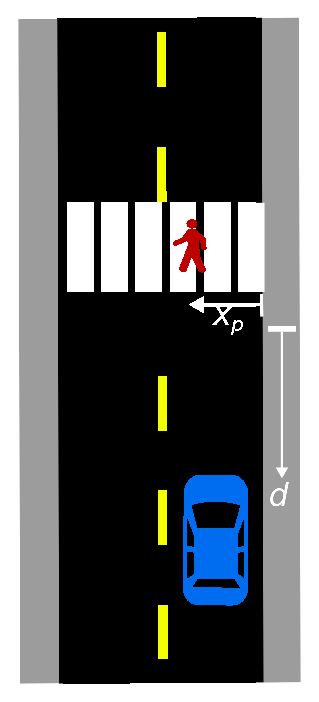
\includegraphics[width=1in]{figures/diagram.eps}
\caption{Description of relevant problem variables.}
\label{fig:diagram1}
\end{figure}

The relevant control problem is therefore to determine an appropriate longitudinal acceleration command for the vehicle, $u = \ddot{d}$, as a closed-loop function of the vehicle and pedestrian states:

\begin{equation}
\ddot{d} = f(d, \dot{d}, x_p, \dot{x_p})
\end{equation}

In general, this control problem is difficult as there are multiple stakeholders and therefore multiple competing objectives that must be considered. For example, relevant stakeholders for this problem are the autonomous vehicle and its passengers, the pedestrian(s), and the other vehicles in the traffic stream. 

As a result, an algorithm that simply yields every time a pedestrian is near the crosswalk is likely to be too conservative, as there is a likelihood the pedestrian is waiting for a larger gap in the traffic stream to cross or is walking through the sidewalk without intending to cross in the first place. To formalize the system requirements for this multi-stake holder problem, we propose the following \textit{design constraints}, extended from the engineering specifications proposed by Thornton \cite{Thornton2018}. 

\begin{center}
\begin{tabular}{ l| l }
\label{tb:specs}
 \textbf{Engineering} & \textbf{Design} \\
 \textbf{Specification} & \textbf{Constraint}\\\hline 
 1. Safety and Legality & a. Avoid collisions for all\\
                     & possible accepted gaps                        \\
                     &b. Ability to follow stop/yield    \\
                     &laws for all 50 U.S. states\\
                     
&\\
 2. Efficiency & a. Average speed: Minimize  \\ 
               & deviation from speed of traffic \\    
               & b. Wait for pedestrian crossing \\
               & event to materialize before yielding. \\ 

               & \\
 3. Smoothness & a. Low accel: Nominal brake / \\ 
 			   & accel limits of 2 m/s/s \\
 			   & b. Stop within 3-5 meters\\
 			   & of crosswalk

\end{tabular}
\end{center}

\section{Proposed Control Architecture}

The proposed control architecture is shown below in Fig.~\ref{fig:hybridController}, and the algorithm for operation is shown in Algorithm \ref{alg:hybridController}. At heart, the control algorithm uses a feedback-feedforward methodology to compute desired acceleration commands $\ddot{d}$, but computes these commands differently depending on which of four discrete states the controller is in. The next sections will describe the four states. 

\begin{figure}
\centering
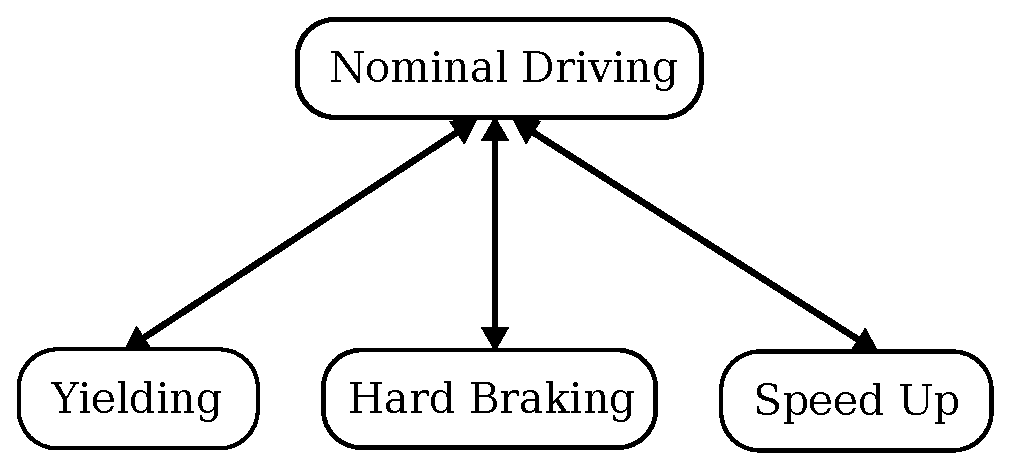
\includegraphics[width=3.5in]{figures/stateDiagram.eps}
\caption{Schematic of hybrid control structure.}
\label{fig:hybridController}
\end{figure}

\begin{algorithm} % enter the algorithm environment
\caption{Calculate $\ddot{d} = f(d, \dot{d}, x_p, \dot{x}_p)$} % give the algorithm a caption
\label{alg:hybridController} % and a label for \ref{} commands later in the document
\begin{algorithmic}
\State $state \leftarrow DRIVING$
\While {$\mathbf{true}$}
\If {$state = DRIVING$}
	\State $\ddot{d} \gets k_s(\dot{d}-v_\mathrm{speed limit})$ 
	\If{$d > 0 \hspace{1mm} \mathbf{and} \hspace{1mm} \mathrm{inCrosswalk}(x_p)$}
		\If{$\mathrm{timeAdvantage}(x_p, \dot{x_p}, d, \dot{d}) > t_{max}$} 
		\State $state \leftarrow DRIVING$
		
		\ElsIf{$d > \frac{\dot{d}^2}{2a_\mathrm{cmfrt}}$}
		\State $state \leftarrow YIELDING$

	\ElsIf{$d < \frac{\dot{d}^2}{2a_\mathrm{cmfrt}} \hspace{1mm} \mathbf{and} \hspace{1mm} d > \frac{\dot{d}^2}{2a_\mathrm{max}}$}
	\State $state \leftarrow HARD\hspace{1mm}BRAKING$

	\Else
	\State $state \leftarrow SPEED\hspace{1mm}UP$

	\EndIf
	\EndIf
	\EndIf
\vspace{3mm}
\If {$state = YIELDING$}
\If {$d > \frac{\dot{d}^2}{2a_\mathrm{cmfrt}} + t_{delay}\dot{d}$}
	\State $\ddot{d}_{des} = 0$
	\State $\dot{d}_{des} = v_\mathrm{speed limit}$
\Else 
	\State $\ddot{d}_{des} = -a_\mathrm{cmf}$
	\State $\dot{d}_{des} = \mathrm{getDesiredSpeed}(d, \dot{d})$
\EndIf 
	\State $\ddot{d} = \ddot{d}_{des} + k_s(\dot{d} - \dot{d}_{des})$

\If {$\textbf{not} \hspace{1mm} \mathrm{inCrosswalk}(x_p)$} \State $state \leftarrow DRIVING$

\EndIf
\EndIf

\vspace{3mm}

\If {$state = HARD\hspace{1 mm}BRAKING$}
	\State $\dot{d}_{des} = \mathrm{getDesiredSpeed}(d, \dot{d})$
	\State $\ddot{d} = -\frac{\dot{d}^2}{2d} + k_s(\dot{d} - \dot{d}_{des})$ 	
	\If {$\textbf{not} \hspace{1 mm} \mathrm{inCrosswalk}(x_p)$} \State $state \leftarrow DRIVING$

	\EndIf
	\EndIf


\EndIf
\If {$state = SPEED\hspace{1mm}UP$}
	\State $\ddot{d} = a_\mathrm{cmf}$ 	
	\If {$\textbf{not} \hspace{1mm} \mathrm{inCrosswalk}(x_p)$} \State $state \leftarrow DRIVING$

	\EndIf
	\EndIf


\EndWhile

\end{algorithmic}
\end{algorithm}

\subsection{Nominal Driving}
In the nominal state, the vehicle attempts to drive through the crosswalk at the speed limit $v_\mathrm{speedlimit}$. A simple proportional speed control is applied to keep the vehicle at the speed limit, achieving design constraint 2.a.:

\begin{equation}
	\ddot{d} = k_s(\dot{d} - v_\mathrm{speedlimit})
\end{equation}

The controller remains in the driving mode unless the pedestrian begins to enter the crosswalk while $d > 0$. To allow more time for the controller to respond, we allow the $\mathrm{inCrosswalk}(x_p, \dot{x}_p)$ indicator function to be triggered the moment the pedestrian approaches the crosswalk from the sidewalk - e.g. once the pedestrian velocity $\dot{x}_p$ becomes non-zero. 

 Note that according to design constraint 1.b, the definition of entering the crosswalk will vary according to which of the fifty US states the vehicle is in. For example, in California, the pedestrian entering any portion of the crosswalk should trigger the control mode to change - while in Louisiana, the pedestrian entering the same half of the roadway as the vehicle should trigger the change \cite{NCSL2018}.  

Once the pedestrian enters the crosswalk, the algorithm decides which mode to enter next. 

\subsubsection{Time Advantage}

Frequently he vehicle will pass through the intersection well before the pedestrian will reach the vehicle's lane. Assuming the vehicle is operating in a US state where stopping is not explicitly required, design constraint 2.a suggests it is desirable for the vehicle to continue through the intersection.

This can be formalized by calculating the \textit{time advantage} $t_adv$, also known as the \textit{time to collision} as follows:

\begin{equation}
t_{adv} = \frac{d}{\dot{d}} - \frac{x_v - x_p}{\dot{x_p}}
\end{equation}

Where $x_v$ is the $x$ position of the vehicle in the crosswalk. The control algorithm in this work will explicitly allow the vehicle to continue driving through the intersection as long as $t_{adv}$ exceeds a specfiied threshold $t_{max}$. 

\subsubsection{Yielding}

If the time advantage is not sufficient for the vehicle to pass through, the autonomous vehicle must slow down. The preferred option to meet design constraint 3.a is to brake at a low, comfortable deceleration $-a_{cmf}$ for the passenger. Note that design constraint 3.b is satisfied by having $d=0$ be defined to be a point several meters ahead of the crosswalk. 

Comfortable braking at a deceleration $-a_{cmf}$ is possible if sufficient braking distance exists. The braking distance is derived kinematically as 

\begin{equation}
d_{brake} = \frac{\dot{d}^2}{2a_{cmf}}
\end{equation}

If this holds true when the pedestrian starts to enter the crosswalk, the car enters a $Yielding$ state. 

\subsubsection{Hard Braking}

In the unlikely event a pedestrian begins to cross when the time gap is low (e.g. under 3 seconds), the vehicle will need to prioritize design constraint 1.a and come to a stop at a deceleration higher than $-a_{cmf}$. This occurs when the following conditions holds:

\begin{equation}
\frac{\dot{d}}{2a_{max}} < d < \frac{\dot{d}^2}{2a_{cmf}}
\end{equation}

Where $a_{max}$ is the largest deceleration magnitude allowed by the tire-road friction. 

\subsection{Speeding Up}

As a final condition, consider the case where the pedestrian enters the crosswalk just as the vehicle is crossing $d = 0$ - in this case, it makes little sense to decelerate, as the vehicle has insufficient space to stop before the crosswalk and will risk being rear-ended (Design Constraint 2.a) or stopping in the crosswalk. It makes more sense in this condition for the vehicle to speed up and exit the crosswalk quickly. As a result, if $d < \frac{\dot{d}}{2a_{max}}$, the vehicle speeds up. 

\subsection{Yielding}

In the yielding state, the vehicle follows a different version of the feedback-feedforward dynamics. The vehicle first follows the speed limit until it reaches the critical value of $\frac{\dot{d}^2}{2a_{cmf}}$. In practice, an additional term $t_delay\dot{d}$ is added to compensate for the delay in brake communication. 

At the critical istance, the vehicle decelerates at the uniform yielding deceleration of $-a_{cmf}$, with an additional feedback term $k_s(\dot{d} - \dot{d}_des$), where $\dot{d}_des$ is the desired velocity. The feedback term helps bring the vehicle speed to 0 at the desired stopping point. 

The desired velocity profile $\dot{d}(d)$ for a vehicle decelerating at constant acceleration is given via integration: 

\begin{equation}
\dot{d}(d) = \sqrt{2a_{cmf}(d-d_o) + \dot{d}_o^2}
\end{equation}

Where $d_o$ and $\dot{d}_o$ is the value of $d$ and $\dot{d}$ when the controller first enters the yielding state. Simple inspection shows that the desired velocity is $\dot{d}_o$ when $d = d_o$ and is 0 when $d = 0$ (recall that we enter the yielding state when $d_o = \frac{\dot{d_o}^2}{2a_{cmf}}$. 

The controller exits the yielding mode and returns to the driving mode once the pedestrian clears the crosswalk. 

\subsection{Hard Braking}

In the hard braking state, the vehicle follows a similar feedback-feedforward algorithm, but the desired feedforward deceleration in this case is given by $\ddot{d} = -\frac{d^2}{2d}$. Integrating to find the desired speed profile $\dot{d}(d)$ yields the following deceleration: 

\begin{equation}
\dot{d}(d) = \frac{\dot{d}_o}{\sqrt{d_o}}\sqrt{d}
\end{equation}     

Where $d_o$ and $\dot{d}_o$ is the value of $d$ and $\dot{d}$ when the controller first enters the braking state. Again, the controller exits the braking mode and returns to the driving mode once the pedestrian clears the crosswalk. 

\subsection{Speed Up}

In the speed up state, there is no need to follow an exact speed profile as the vehicle is merely trying to exit the crosswalk area slightly faster. In this case, the commanded acceleration $\ddot{d} = a_{cmf}$ until the pedestrian clears the crosswalk. 

\section{Evaluation Methodology and Simulation Results}

\subsection{Evaluation Methodology}

In order to check performance of the algorithm, both simulation and experimental studies were undertaken. The simulation results focused on testing Algorithm 1 against the design requirements from Table \ref{tb:specs} over many pedestrian crossings. 

The algorithm is validated in simulation via a built-from-scratch crosswalk simulation environment (Fig. \ref{fig:simFramework}) developed in Python. The simulation environment is built on the ROS \cite{ROS} robotics interface to enable easy porting of the control architecture to the experimental vehicle in Section \ref{sec:expres}. The simulation includes features such as multiple lanes, the pedestrian crossing on the right or the left, and animation capabilities.    

\begin{figure}
\centering
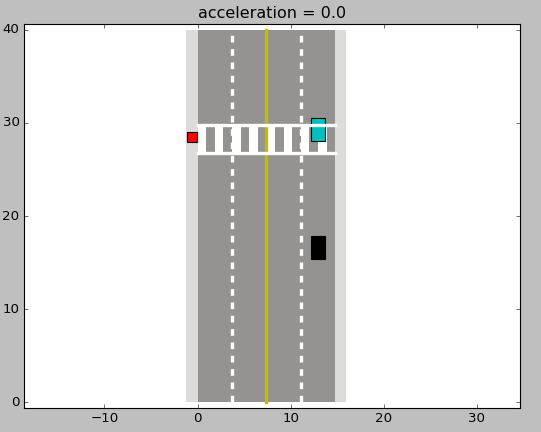
\includegraphics[width=2.5in]{figures/simFramework.png}
\caption{Crosswalk simulation environment for algorithm validation. Ego vehicle is shown in black, following vehicle in traffic stream shown in blue, and pedestrian shown in red.}
\label{fig:simFramework}
\end{figure}

To simulate random pedestrian crossing events, a pedestrian is spawned in an area near the crosswalk. The pedestrian accepts a randomly sized time gap in the traffic stream to cross the road at constant speed $\dot{x}_p$. The size of the time gap is drawn from a normal distribution with mean $\mu_{gap}$ and standard deviation $\sigma_{gap}$. Statistics for $\mu_{gap}$ and $\sigma_{gap}$ are obtained from a video graphic analysis by Feliciani et al. \cite{Feliciani2017}. 

The ego vehicle's response to the pedestrian is simulated over Algorithm 1 for the parameters shown in Table \ref{tb:params}.  

\begin{table}[h]
\footnotesize
\begin{center}
\caption{Simulation and Controller Parameters}\label{tb:params}
\begin{tabular}{lccc}
Parameter & Symbol & Value & Units \\\hline\hline
Number of lanes & $n$ & 4 & - \\
Gap variance & $\sigma_{gap}$ & 2.5 & sec\\
Mean accepted gap & $\mu_{gap}$ & 4.0 & sec\\\hline
Speed feedback gain & $k_s$ & 2.0 & 1 / sec\\
Brake time delay    & $t_\mathrm{delay}$ & 0 & sec \\ 
Speed limit & $v_\mathrm{speedlimit}$ & 4.5 & m/s \\
Comfort acceleration & $a_\mathrm{cmf}$ & 2 & $\mathrm{m/s^2}$ \\
Maximum time advantage & $t_\mathrm{max}$ & 4 & sec \\
Maximum acceleration & $a_\mathrm{max}$ & 9 & $\mathrm{m/s^2}$ \\\hline
\end{tabular}
\end{center}
\end{table}

\subsection{Simulation Results}

Figure \ref{fig:velPlot1} shows simulation results for the case where the pedestrian enters the crosswalk on the same side of the road as the vehicle. The left side of the figure is for the case where the vehicle is on the right-most lane of a four way road, while the right side of the figure is for the case where the vehicle is in the second to right lane. Every marker in the figure represents a simulated vehicle crossing.

\begin{figure}
\centering
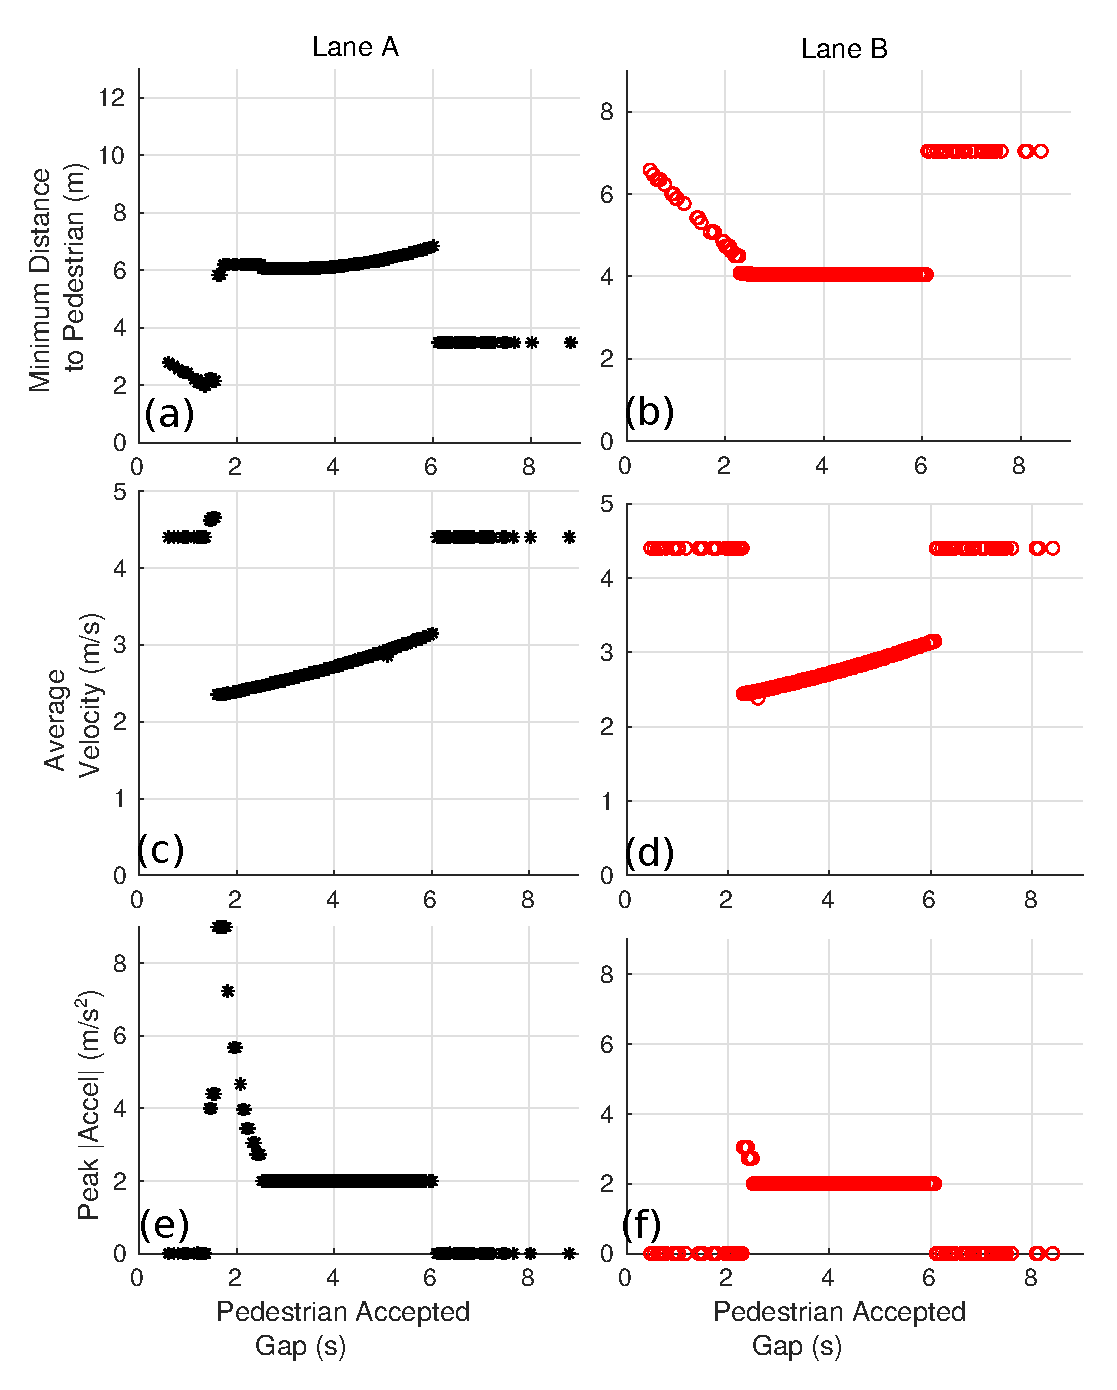
\includegraphics[width=3.5in]{figures/velPlot.eps}
\caption{Simulation results for case where pedestrian enters the crosswalk on the same side of the road as the vehicle.}
\label{fig:velPlot1}
\end{figure}

Figure \ref{fig:velPlot2} shows the same simulation results, but for the case where the pedestrian enters the crosswalk on the opposite side of the road as the vehicle. Again, the total number of pedestrian crossing trials conducted was 750, with 375 trials for each side.  

\begin{figure}
\centering
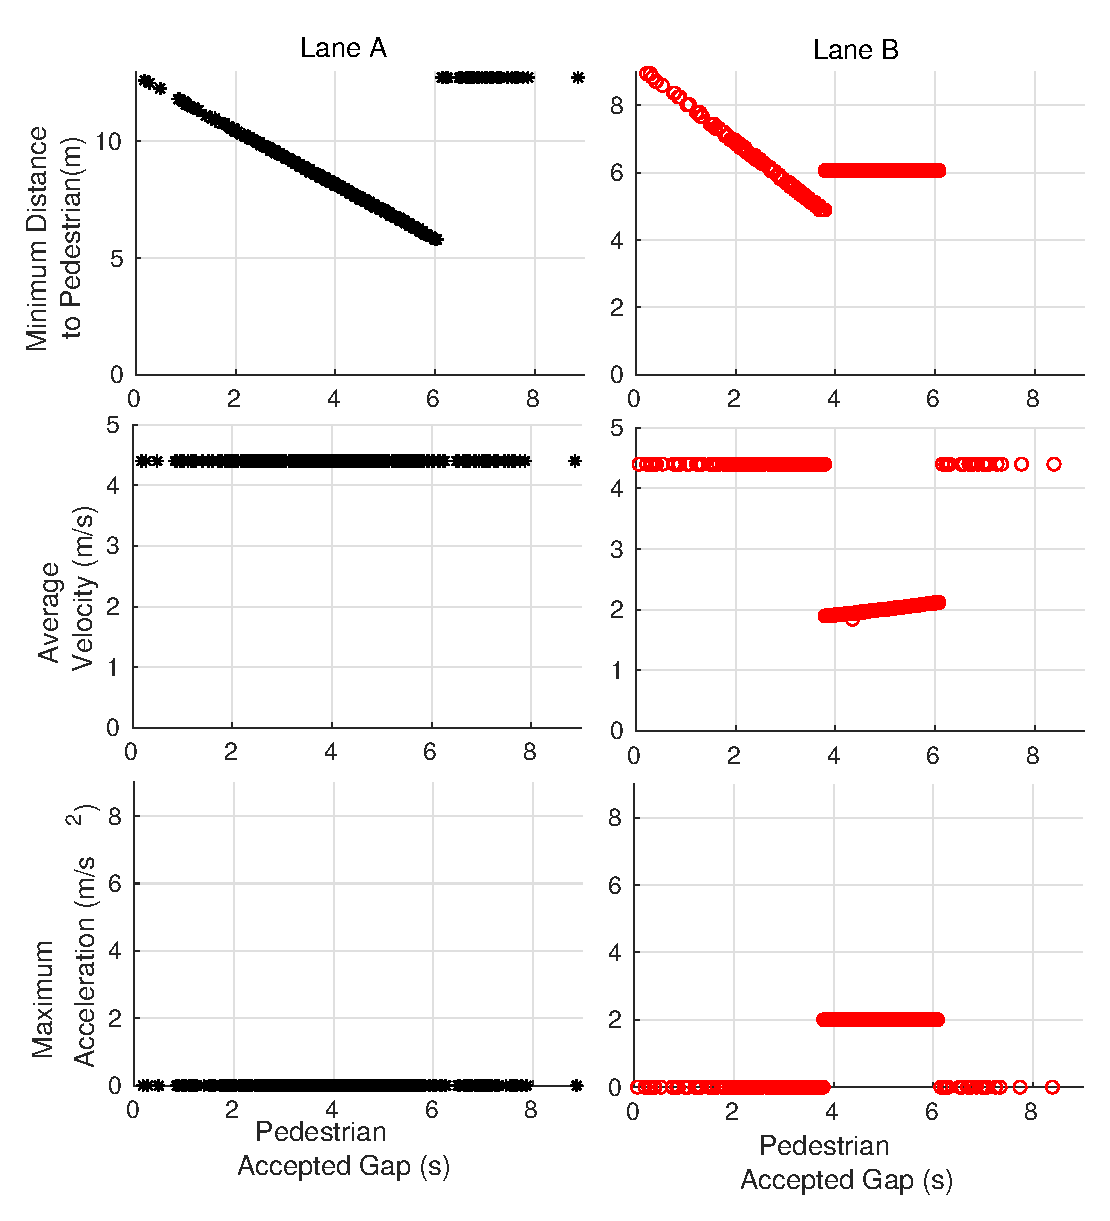
\includegraphics[width=3.5in]{figures/velPlot2.eps}
\caption{Simulation results for case where pedestrian enters the crosswalk on the opposite side of the road as the vehicle.}
\label{fig:velPlot2}
\end{figure}

\subsubsection{Safety and Legality}

To meet the collision avoidance design requirement, we generated enough simulations to ensure errant pedestrian crossing behavior at "risky" accepted gaps (< 3 seconds). The minimum distance between the vehicle and the pedestrian for each trial is shown in the bottom rows of Fig. \ref{fig:velPlot1} and Fig.\ref{fig:velPlot2}. In general, the vehicle is able to maintain a safe distance of at least four meters from the pedestrian for the case where the vehicle is in the second to right lane. This is because the algorithm has enough time to react to a pedestrian crossing no matter what size gap is accepted. 

The riskiest case occurs when the vehicle is in the right-most lane and the pedestrian crosses from the right side, accepting a gap between 1.25 and 1.75 seconds. Note that this is in general unlikely given gap acceptance statistics reported in the literature \cite{Feliciani2017}\cite{Rasouli}, but would represent a safety risk given the vehicle has limited time to react. However, since the algorithm recognizes that braking will not clear the crosswalk, the vehicle is able to speed up and maintain at least 2 meters of lateral distance from the pedestrian at all times. Note that a better way to confirm robustness of the controller to all reasonable pedestrian behaviors would be through a verification analysis - this will be the focus of future work. 

In terms of the fifty state legality requirement, we conducted our simulation for the twenty states where the vehicle is required to yield, not stop, to a pedestrian in the same side of the crosswalk or approaching from the opposite side. For the US states where the vehicle is explicitly required to stop, the change to the controller is trivial - the controller may not stay in the driving mode if sufficient time advantage exits (see Algorithm 1). 

\subsubsection{Efficiency}

The requirement to minimize deviation from speed of traffic is validated in the top row of Fig.\ref{fig:velPlot1} and Fig.\ref{fig:velPlot2}, which shows the average velocity of the vehicle for each simulated crossing. For high accepted gaps, the pedestrian simply waits for the ego vehicle to exit the crosswalk before beginning to walk, and the algorithm does not need to slow down from the speed of traffic. For low accepted gaps, the vehicle cannot stop, and must speed up or continue driving through the intersection, also keeping the speed of traffic high.  

The most disruption to traffic flow occurs when the vehicle must come to a complete stop, which occurs for accepted gaps between 2-6 seconds. In this case, the average velocity increases as the accepted gap increases. This is because as the pedestrian enters the crosswalk earlier, they are closer to exiting when the vehicle must yield, resulting in less time stopped and higher average velocity. 

Note that a special case occurs in Fig.\ref{fig:velPlot2} where the vehicle is in the right-most lane of the four lane road and the pedestrian crosses from the other side. Because the vehicle is at a far distance from the pedestrian, the time advantage remains sufficiently high for the vehicle to comfortably continue through the crosswalk without needing to slow down. 

Table \ref{tb:speeds} shows a summary of the average speed compared to the baseline speed of 4.4 m/s.

\begin{table}[h]
\footnotesize
\begin{center}
\caption{Average Vehicle Speed}\label{tb:speeds}
\begin{tabular}{cccc}
Pedestrian Entry & Vehicle Lane & Average Speed (m/s) & Pct. of Baseline \\\hline\hline

Right Side & Right-Most & 2.90 & 66\% \\
Right Side & Second-to-Right & 2.93 & 67\% \\
Left Side  & Right-Most & 4.4 & 100\% \\
Left Side  & Second-to-Right & 2.80 & 64\% \\\hline

\end{tabular}
\end{center}
\end{table}

\subsubsection{Smoothness}
The requirement of keeping a low acceleration where possible is validated through the middle rows of Fig.\ref{fig:velPlot1} and Fig.\ref{fig:velPlot2}.The vehicle is able to maintain a peak acceleration of 2 $\mathrm{m/s^2}$ for the vast majority of simulated trials, particularly when the pedestrian crosses from the opposing side of the road or when the vehicle is in the second to right line.

However, there are a handful of simulated trials in Fig.\ref{fig:velPlot1} when the pedestrian accepts a gap between 1.75-2.5 seconds and the vehicle is in the right-most lane closest to the sidewalk. In this case, the vehicle must enter the \textit{Hard Braking} state and decelerate at a magnitude higher than $a_\mathrm{cmf}$. This is required in order to meet the collision avoidance constraint, which naturally takes priority. Again, note that this situation occurs relatively rarely, as pedestrians typically accept gaps between 3-6 seconds and are unlikely to risk hazardous behaviors unless distracted. 

\begin{figure}[h]
\centering
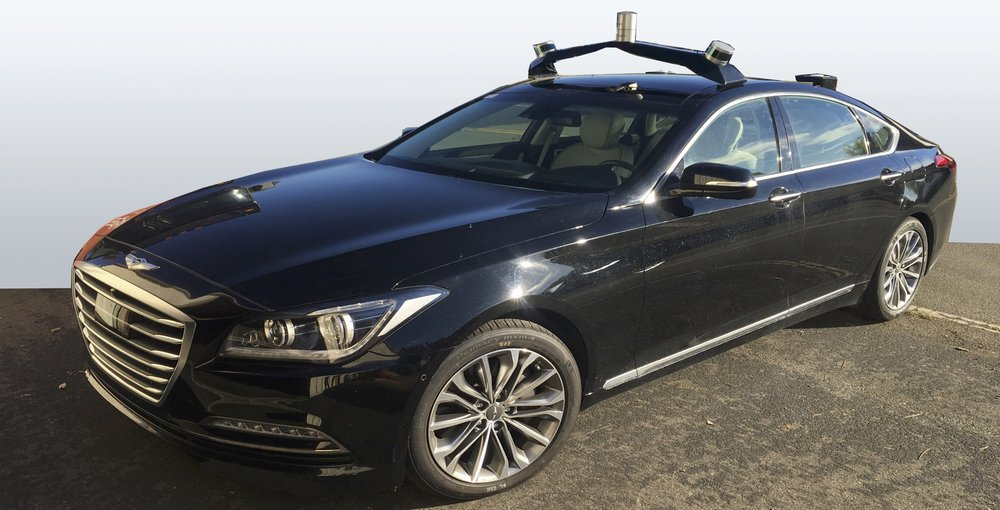
\includegraphics[width=3.0in]{figures/G80.jpg}
\caption{Hyundai Genesis G80 experimental testbed.}
\label{fig:g80}
\end{figure}


\section{Experimental Results}
\label{sec:expres}


The proposed hybrid controller is tested experimentally using a Hyundai Genesis G80 experimental testbed, shown in Fig. \ref{fig:g80}. A mid-block intersection at Richmond Field Station near Berkeley's campus was chosen for the experimental validation.  In lieu of an actual pedestrian, a pedestrian was simulated virtually using the ROS simulation architecture described earlier, with the position of the pedestrian sent to the vehicle in real time. Differential GPS was used to record the distance to the crosswalk, and a steering controller from \cite{kapania} was used to autonomously steer the vehicle in a straight line path. Relevant parameters of the experiments are shown below in Tables \ref{tb:expparams}.

\begin{table}[h]
\footnotesize
\begin{center}
\caption{Experimental Parameters}\label{tb:expparams}
\begin{tabular}{lccc}
Parameter & Symbol & Value & Units \\\hline\hline
Number of lanes & $n$ & 2 & - \\
Speed feedback gain & $k_s$ & 2.0 & 1 / sec\\
Brake time delay    & $t_\mathrm{delay}$ & 0.5 & sec \\ 
Speed limit & $v_\mathrm{speedlimit}$ & 7 & m/s \\
Comfort acceleration & $a_\mathrm{cmf}$ & 2 & $\mathrm{m/s^2}$ \\
Maximum time advantage & $t_\mathrm{max}$ & 4 & sec \\
Maximum acceleration & $a_\mathrm{max}$ & 9 & $\mathrm{m/s^2}$ \\\hline
\end{tabular}
\end{center}
\end{table}

Several key differences to highlight between the simulations and the experiments are that the number of lanes is decreased from 4 to 2 and that the speed limit is increased to 7 m/s to match the parameters of the experimental intersection. The experiment consisted of six trials intended to show operation of the four discrete modes of the controller. A description of the trial parameters are shown in Table \ref{tb:expparams2}. 


\begin{table}[h]
\footnotesize
\begin{center}
\caption{Experimental Parameters}\label{tb:expparams2}
\begin{tabular}{llll}
Trial Number & Gap Accepted (sec) & Pedestrian Entry & Mode\\\hline\hline
1 & 4.0 & right &  Yield\\ 
2 & 1.0 & right &  Speed Up\\ 
3 & 7.0 & right &  Yield\\ 
4 & 2.5 & right &  Hard Brake\\ 
5 & 3.0 & left  &  Yield \\ 
6 & 1.0 & left  &  Speed Up\\\hline
\end{tabular}
\end{center}
\end{table}

The experimental velocity and acceleration is plotted vs $d$ in 
Figure \ref{fig:diagram1}. In Trial 1, the virtual pedestrian enters when the vehicle is four seconds from intersecting, giving the vehicle enough time to yield at a deceleration of 2 $m/s^2$. Note that the vehicle exhibits a large time delay between commanded and actual acceleration. Because this is accounted for in Algorithm 1, the vehicle is able to brake early and the vehicle is nearly stopped at $d = $ 1 meter before the pedestrian exits the crosswalk and the vehicle speeds back up. This overshoot, while undesirable, is realistically acceptable given the point $d=0$ is set to be several meters before the crosswalk actually begins. 

\begin{figure}[h]
\centering
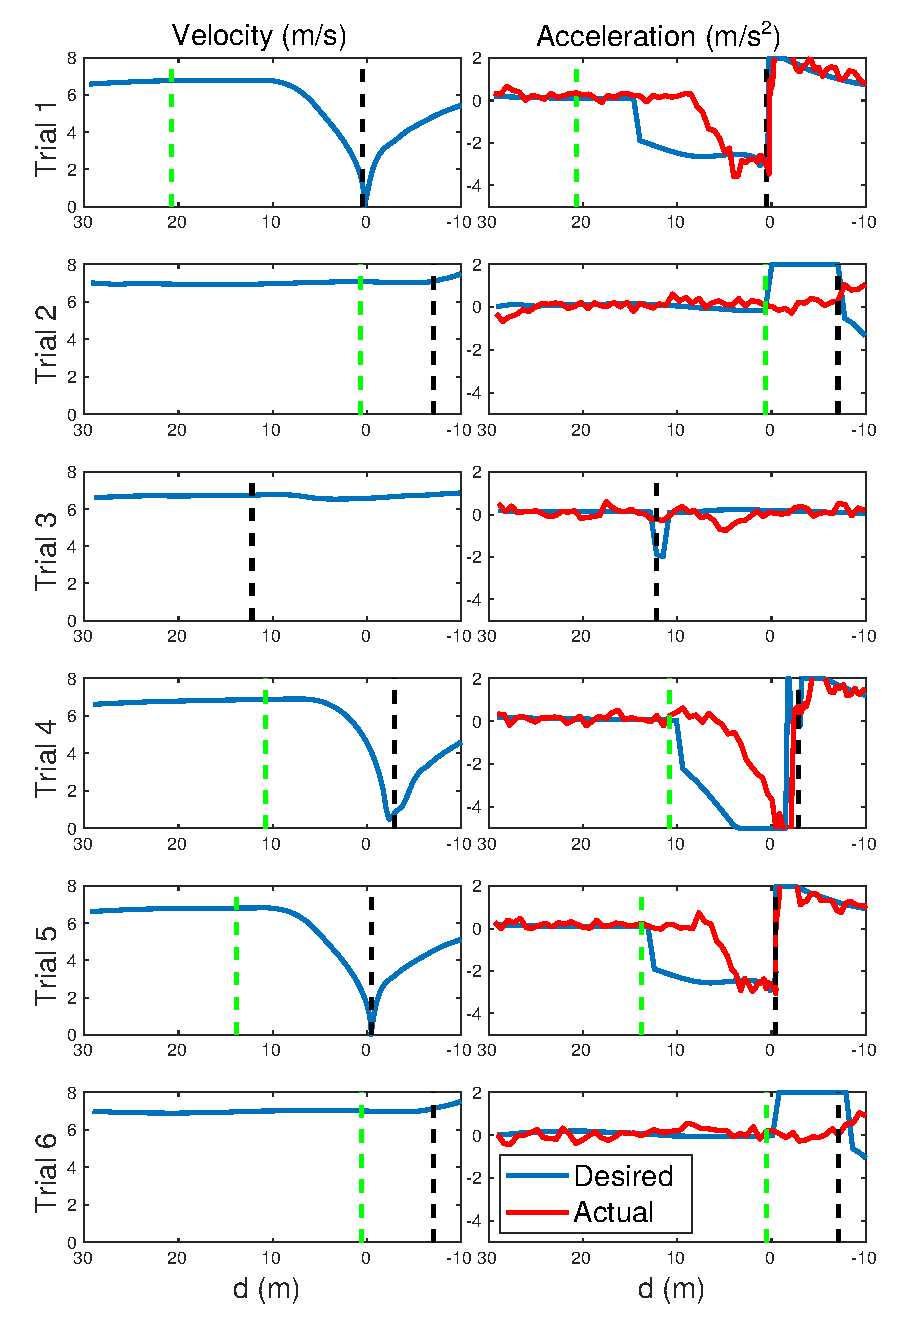
\includegraphics[width=3.5in]{figures/expPlot.eps}
\caption{Experimental velocity and acceleration plotted vs distance to crosswalk. Note that the sign of $d$ is opposite that of Fig.\ref{fig:diagram1}}
\label{fig:g80}
\end{figure}

In Trial 2, the pedestrian enters from the right with just 1 second before collision. This experiment, while unlikely in reality, was undertaken to verify the vehicle would not brake, but accelerate through the intersection. Trial 3 represents a situation where the pedestrian crosses with a large (7 second) gap. In this case, the pedestrian has enough time to almost cross before the vehicle needs to yield, resulting in the vehicle only needing to slow down slightly. 

In Trial 4, the pedestrian exhibits risky behavior, crossing with a 2.5 second gap. In this case, the vehicle has enough time to brake, but must decelerate rapidly at 5 $m/s^2$ in the \textit{hard braking} mode. Given the brake delay in the experimental vehicle, significant overshoot occurs, and the vehicle stops nearly 2.5 meters ahead of the desired stopping location. Unlike in the yielding mode, the brake delay can not be compensated for because the vehicle must brake suddenly. 

Trials 5 and 6 represent pedestrian crossings from the opposite side of the road under accepted gaps of 3.0 and 1.0 seconds, respectively. In the former case, the vehicle is able to yield in a fashion similarly to Trial 1, and in the latter case, the vehicle is able to speed through the intersection, as in Trial 2. 

\section{CONCLUSIONS}


\addtolength{\textheight}{-12cm}   % This command serves to balance the column lengths
                                  % on the last page of the document manually. It shortens
                                  % the textheight of the last page by a suitable amount.
                                  % This command does not take effect until the next page
                                  % so it should come on the page before the last. Make
                                  % sure that you do not shorten the textheight too much.

%%%%%%%%%%%%%%%%%%%%%%%%%%%%%%%%%%%%%%%%%%%%%%%%%%%%%%%%%%%%%%%%%%%%%%%%%%%%%%%%



%%%%%%%%%%%%%%%%%%%%%%%%%%%%%%%%%%%%%%%%%%%%%%%%%%%%%%%%%%%%%%%%%%%%%%%%%%%%%%%%



%%%%%%%%%%%%%%%%%%%%%%%%%%%%%%%%%%%%%%%%%%%%%%%%%%%%%%%%%%%%%%%%%%%%%%%%%%%%%%%%
\section*{APPENDIX}

Appendixes should appear before the acknowledgment.

\section*{ACKNOWLEDGMENT}





%%%%%%%%%%%%%%%%%%%%%%%%%%%%%%%%%%%%%%%%%%%%%%%%%%%%%%%%%%%%%%%%%%%%%%%%%%%%%%%%



\bibliographystyle{IEEEtran}
\bibliography{Bibliography}




\end{document}
